\section{Phénoménologie des événements photon + jets}
$\photon+\text{jet}$ donne beaucoup de stats, donc on peut sélectionner beaucoup et obtenir une bonne pureté.
\begin{figure}[h]
\centering\vspace{\baselineskip}
\subcaptionbox{\label{subfig-fgraph-gq_qGamma_S}}[.25\textwidth]
{\begin{fmffile}{gq_qGamma_S}\fmfstraight
\begin{fmfchar*}(20,20)
  \fmfleft{i1,i2}
  \fmfright{o1,o2}
  \fmf{gluon}{i2,v1}
  \fmf{fermion}{i1,v1,v2,o2}
  \fmf{photon}{v2,o1}
  \fmflabel{\gluon}{i2}
  \fmflabel{\quark}{i1}
  \fmflabel{\quark}{o2}
  \fmflabel{\photon}{o1}
  \fmfdot{v1,v2}
\end{fmfchar*}
\end{fmffile}}
\qquad
\subcaptionbox{\label{subfig-fgraph-gq_qGamma_T}}[.25\textwidth]
{\begin{fmffile}{gq_qGamma_T}\fmfstraight
\begin{fmfchar*}(20,20)
  \fmfleft{i1,i2}
  \fmfright{o1,o2}
  \fmf{gluon}{i2,v2}
  \fmf{fermion}{i1,v1,v2,o2}
  \fmf{photon}{v1,o1}
  \fmflabel{\gluon}{i2}
  \fmflabel{\quark}{i1}
  \fmflabel{\quark}{o2}
  \fmflabel{\photon}{o1}
  \fmfdot{v1,v2}
\end{fmfchar*}
\end{fmffile}}
\qquad
\subcaptionbox{\label{subfig-fgraph-qq_gGamma}}[.25\textwidth]
{\begin{fmffile}{qq_gGamma}\fmfstraight
\begin{fmfchar*}(20,20)
  \fmfleft{i1,i2}
  \fmfright{o1,o2}
  \fmf{gluon}{v2,o2}
  \fmf{fermion}{i1,v1,v2,i2}
  \fmf{photon}{v1,o1}
  \fmflabel{\antiquark}{i2}
  \fmflabel{\quark}{i1}
  \fmflabel{\gluon}{o2}
  \fmflabel{\photon}{o1}
  \fmfdot{v1,v2}
\end{fmfchar*}
\end{fmffile}}
\caption{Exemples de diagrammes de Feynman de processus physiques donnant un photon et un jet dans l'état final.}
\label{fig-fgraph-gamma_plus_jets}
\end{figure}

\begin{figure}[h]
\centering
\subcaptionbox{\label{subfig-Gamma_plus_jet_basic_event}}[.45\textwidth]
{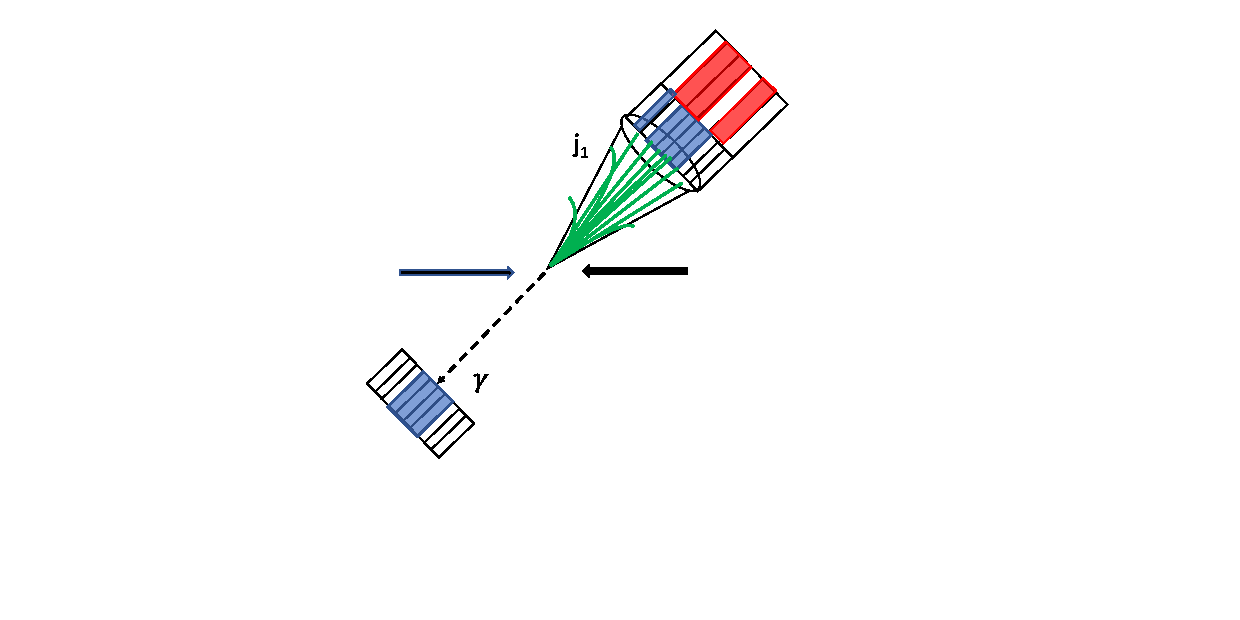
\includegraphics[width=\linewidth,height=.25\textheight,keepaspectratio, trim = 5cm 2.5cm 7.5cm .5cm, clip]{\PhDthesisdir/tex/slides/JERC/JEC_Principe/Gamma_plus_jet_basic_event.pdf}}
\qquad
\subcaptionbox{\label{subfig-Gamma_plus_two_jets}}[.45\textwidth]
{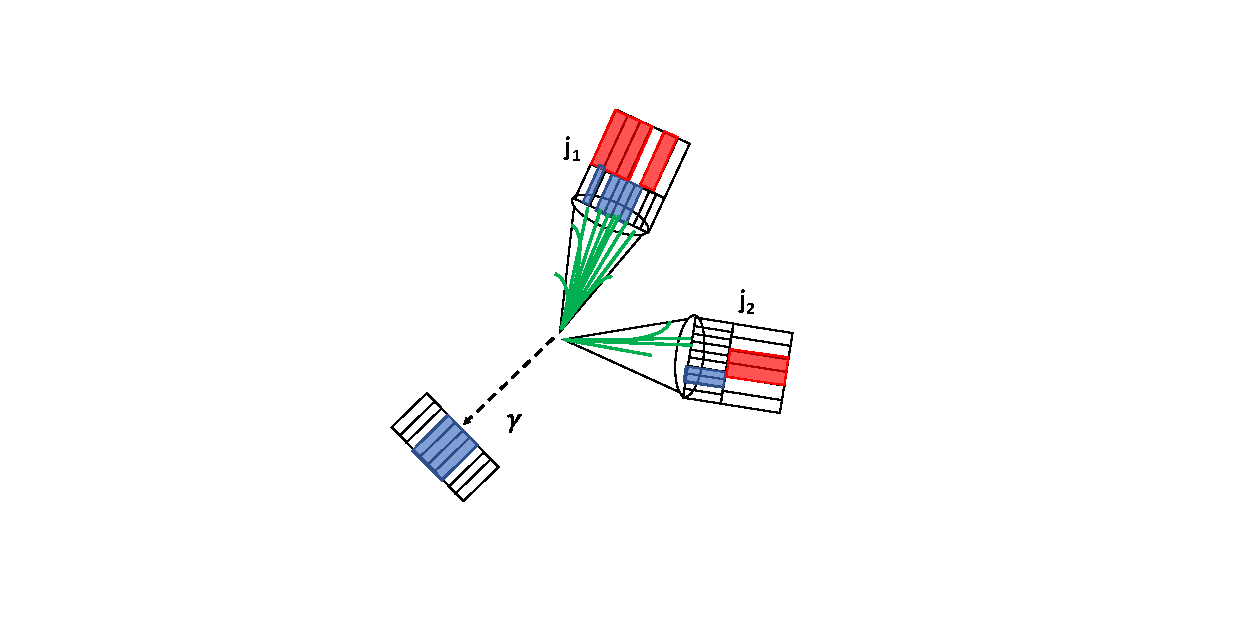
\includegraphics[width=\linewidth,height=.25\textheight,keepaspectratio, trim = 5.5cm 2cm 7.5cm 1.75cm, clip]{\PhDthesisdir/tex/slides/JERC/JEC_Principe/Gamma_plus_two_jets.pdf}}
\caption{•}
\label{fig-Gamma_plus_jet_events}
\end{figure}

initial state radiation: réjection par la condition back-to-back.